% Figure of the starter poster (scripts/gen-starters.ts compiles it to templates/starters/poster/figures/results.pdf).
\documentclass[border=2pt]{standalone}
\usepackage[T1]{fontenc}
\usepackage[scaled]{helvet}
\renewcommand{\familydefault}{\sfdefault}
\usepackage{sansmath}
\usepackage{pgfplots}
\pgfplotsset{compat=1.18}
\begin{document}
\sansmath
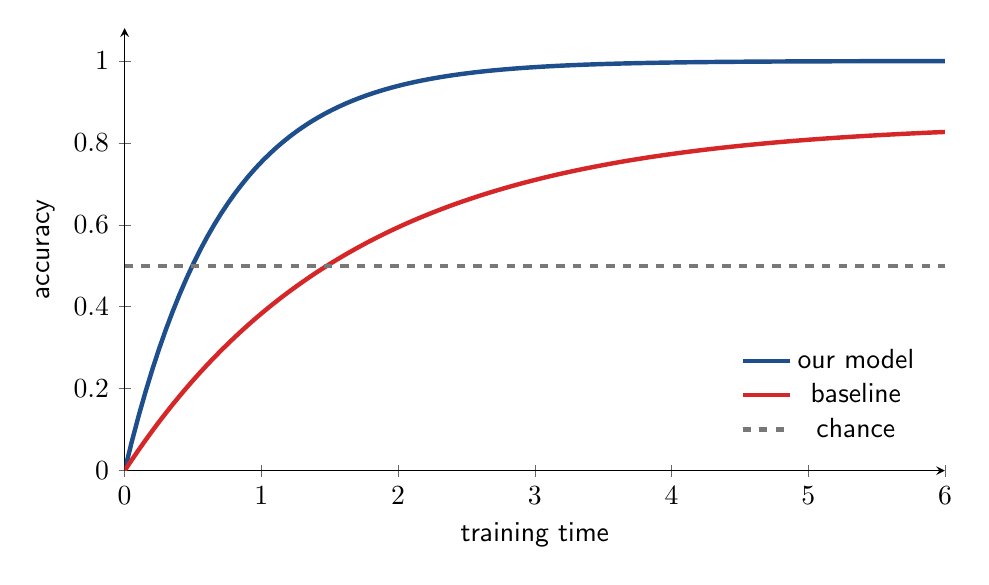
\begin{tikzpicture}
\begin{axis}[width=12cm, height=7.2cm, xmin=0, xmax=6, ymin=0, ymax=1.08,
  xlabel={training time}, ylabel={accuracy}, axis lines=left, tick style={black!60},
  legend style={draw=none, fill=none, at={(0.98,0.04)}, anchor=south east},
  every axis plot/.append style={line width=1.6pt, samples=120, domain=0:6}]
\addplot[color={rgb,255:red,31;green,78;blue,140}] {1-exp(-1.4*x)};
\addplot[color={rgb,255:red,214;green,39;blue,40}] {0.85*(1-exp(-0.6*x))};
\addplot[color={rgb,255:red,120;green,120;blue,120}, dashed, domain=0:6] {0.5};
\legend{our model, baseline, chance}
\end{axis}
\end{tikzpicture}
\end{document}
